% !TeX root = ../../infdesc.tex
\section{Inductively defined sets}
\secbegin{secStructuralInduction}
\index{induction!structural|(}

In \Cref{secPeanosAxioms}, we formalised the idea that the set of natural numbers should be what is obtained by starting with zero and repeating the successor (`plus one') operation---this was done using Peano's axioms (\Cref{defNotionOfNaturalNumbers}). From these axioms we were able to derive the weak and strong induction principles, which turned out to be extremely powerful for proving results about natural numbers.

We now generalise this idea to other so-called \textit{inductively defined} sets. The definition (\Cref{defInductivelyDefinedSet}) is a little tricky to digest, but the idea is relatively simple: an inductively defined set $X$ is one whose elements are built out of some specified \textit{basic elements} (such as $0$) by iterating some specified operations, called \textit{constructors} (such as the successor operation)---every element of $X$ should either be a basic element, or should be built in a unique way out of simpler elements of $X$ by using a constructor.

Each inductively defined set $X$ will have its own induction principle: which says that if a property is true of all of the basic elements of $X$, and if all of its constructors preserve the truth of the property, then the property is true of all of the elements of $X$. We will prove this in \Cref{thmStructuralInduction}.

Before jumping into the definition of an inductively defined set, it is helpful to see some examples. The first example is familiar.

\begin{example}
\label{exNaturalNumbersAsInductivelyDefinedSetPreliminary}
The set $\mathbb{N}$ of natural numbers is \textit{the} canonical example of an inductively defined set. The Peano axioms (\Cref{defNotionOfNaturalNumbers}) tell us that every element of $\mathbb{N}$ can be obtained by starting from $0$ and applying the successor operation (`plus one') some finite number of times. In particular, every natural number is either $0$, or is the successor of a unique natural number.

We can think of $\mathbb{N}$ as being the set \textit{generated by} the following rules:
\begin{enumerate}[(i)]
\item $0 \in \mathbb{N}$; and
\item If $n \in \mathbb{N}$, then $n+1 \in \mathbb{N}$.
\end{enumerate}
Certainly these rules are \textit{true}, but that is not enough to fully characterise the set of natural numbers: both rules are also true with $\mathbb{N}$ replaced by $\mathbb{Z}$ or $\mathbb{R}$, for example.

But what it means to say that $\mathbb{N}$ is `generated by' these rules is that:
\begin{itemize}
\item Each time one of the rules is applied, we obtain a \textit{new} natural number. In particular:
\begin{itemize}
\item Since $0 \in \mathbb{N}$ and rule (ii) must give us a new natural number every time we apply it, we must have $n+1 \ne 0$ for all $n \in \mathbb{N}$. This is exactly what \Cref{defNotionOfNaturalNumbers}(i) says; note that this fails with $\mathbb{N}$ replaced by $\mathbb{Z}$ or $\mathbb{R}$ since we have $(-1)+1 = 0$.
\item If we apply rule (ii) to two different natural numbers, we must obtain two different results. Thus for all $m,n \in \mathbb{N}$, if $m+1=n+1$, then $m=n$. This is exactly what \Cref{defNotionOfNaturalNumbers}(ii) says.
\end{itemize}
\item Only those things that can be obtained by applying rules (i) and (ii) some finite number of times are natural numbers. This is exactly what \Cref{defNotionOfNaturalNumbers}(iii) says.
\end{itemize}

Thus we can think of the natural numbers as being precisely those things that are given to us by applying rules (i) and (ii).
\end{example}

The next example concerns words over an alphabet, which we studied in \Cref{secCountableUncountableSets} in the context of determining when a set is countable---see \Cref{defKleeneStar}.

\begin{example}
\label{exWordsAsInductivelyDefinedSetPreliminary}
Let $\Sigma$ be a fixed alphabet. The set $\Sigma^*$ of words over $\Sigma$ is built by starting from the empty word $\varepsilon$ by appending elements $a \in \Sigma$. Thus $\Sigma^*$ is generated by the following rules:
\begin{enumerate}[(i)]
\item $\varepsilon \in \Sigma^*$; and
\item For all $a \in \Sigma$, if $w \in \Sigma^*$, then $wa \in \Sigma^*$.
\end{enumerate}
The fact that $\Sigma^*$ is \textit{generated by} these rules means that:
\begin{itemize}
\item Each time we append an element $a \in \Sigma$ to the end of a word $w \in \Sigma^*$, the resulting word $wa$ is a new element of $\Sigma^*$; and
\item Only those things obtained by appending elements $a \in \Sigma$ to the end of the empty word $\varepsilon$ some finite number of times are elements of $\Sigma^*$.
\end{itemize}

We can actually think of rule (ii) as being a family of rules, one rule for each $a \in \Sigma$. For fixed $a$, the rule says `for all $w$, if $w \in \Sigma^*$, then $wa \in \Sigma^*$'. This viewpoint is useful because it allows us to restrict our attention to rules that only have variable elements of the set being inductively defined in the hypothesis.
\end{example}

We alluded to the inductive character of propositional formulae in \Cref{secPropositionalLogic}. Although we were not able to make the idea precise at the time, we are now well on our way to doing so.

\begin{example}
\label{exPropositionalFormulaeAsInductivelyDefinedSetPreliminary}
Given a set $P$, consider the set $\mathcal{L}(P)$ of all propositional formulae with propositional variables from $P$ and logical operators from the set $\{ {\wedge}, {\vee}, {\Rightarrow}, {\neg} \}$. Then $\mathcal{L}(P)$ is built out of the elements of $P$ using these logical operators.

Specifically, $\mathcal{L}(P)$ is generated by the following rules:
\begin{enumerate}[(i)]
\item For each $p \in P$, we have $p \in \mathcal{L}(P)$;
\item If $\varphi, \psi \in \mathcal{L}(P)$, then $\varphi \wedge \psi \in \mathcal{L}(P)$;
\item If $\varphi, \psi \in \mathcal{L}(P)$, then $\varphi \vee \psi \in \mathcal{L}(P)$;
\item If $\varphi, \psi \in \mathcal{L}(P)$, then $\varphi \Rightarrow \psi \in \mathcal{L}(P)$;
\item If $\varphi \in \mathcal{L}(P)$, then $\neg \varphi \in \mathcal{L}(P)$.
\end{enumerate}

To say that $\mathcal{L}(P)$ is generated by these rules means that every propositional formula is (exclusively) either: a propositional variable, the conjunction of two simpler formulae, the disjunction of two simpler formulae, the implication formed by two simpler formulae, or the negation of a simper formula.

We can interpret (i) as being a family of rules, one for each $p \in P$, where for fixed $p$, the rule simply says `$p \in \mathcal{L}(P)$'. Just like we said in \Cref{exWordsAsInductivelyDefinedSetPreliminary}, this is useful because it removes variable elements of sets other than $\mathcal{L}(P)$ from the hypotheses of the rule.
\end{example}

Keeping these examples in mind, we will now work towards defining the notion of an \textit{inductively defined set}. First we formalise the notion of a rule.

\begin{definition}
\label{defRuleForInductiveDefinition}
\index{induction!rule}
\index{rule}
A (\textbf{finitary}) \textbf{rule} for an inductive definition is an expression of the form
\[ (\mathbf{x} \mid \sigma(\mathbf{x})) \quad \text{\inlatex{mid}} \]
where $\mathbf{x}$ is a (possibly empty) list of variables, and $\sigma(\mathbf{x})$ is some expression which may involve the variables in $\mathbf{x}$.

The number of variables in $\mathbf{x}$ is called the \textbf{arity} of the rule, and is denoted by $\mathrm{ar}(\sigma)$ \inlatex{mathrm\{ar\}}\lindexmmc{mathrm}{$\mathrm{Aa}, \mathrm{Bb}, \dots$}.
\end{definition}

A quick note on terminology: a constructor of arity $r \in \mathbb{N}$ is called an \textit{$r$-ary} constructor. For $r=0,1,2$, we may say \textit{nullary}, \textit{unary} and \textit{binary}, respectively.

We interpret the rule $(x,y,\dots{} \mid \sigma(x,y,\dots{}))$ as meaning `if $x,y,\dots$ are elements of the set being defined, then $\sigma(x,y,\dots{})$ is an element of the set being defined'.

Note that nullary rules take the form $(~ \mid a)$, where $a$ is some expression with no variables; we would interpret such a rule as saying `$a$ is an element of the set being defined', with no hypotheses.

\begin{example}
The rules describing the natural numbers are $(~ \mid 0)$ and $(n \mid n+1)$. The rule $(~ \mid 0)$ can be interpreted to mean `$0$ is a natural number', and the rule $(n \mid n+1)$ can be interpreted to mean `if $n$ is a natural number, then $n+1$ is a natural number'. In the context of \Cref{exNaturalNumbersAsInductivelyDefinedSetPreliminary}, this means that $(~ \mid 0)$ corresponds with rule (i) and $(n \mid n+1)$ corresponds with rule (ii).
\end{example}

\begin{example}
\label{exRulesForInductiveDefinitionOfPropositionalFormulae}
Let $P$ be a set of propositional variables. The rules that describe the set $\mathcal{L}(P)$ of logical formulae over $P$, as described in \Cref{exPropositionalFormulaeAsInductivelyDefinedSetPreliminary}, are given by
\[ \underbrace{(~ \mid p)}_{\text{one for each } p \in P} \quad (\varphi,\psi \mid \varphi \wedge \psi) \quad (\varphi,\psi \mid \varphi \vee \psi) \quad (\varphi,\psi \mid \varphi \Rightarrow \psi) \quad (\varphi \mid \neg \varphi) \]

The first of these rules says that every propositional variable $p \in P$ is a propositional formula. The next three say that if $\varphi$ and $\psi$ are propositional formulae, then so are $\varphi \wedge \psi$, $\varphi \vee \psi$ and $\varphi \Rightarrow \psi$. The last rule says that if $\varphi$ is a propositional formula, then so is $\neg \varphi$.
\end{example}

\begin{exercise}
\label{exRulesForInductiveDefinitionOfWords}
Fix an alphabet $\Sigma$. Following \Cref{exWordsAsInductivelyDefinedSetPreliminary}, define rules that describe the set $\Sigma^*$ of words over $\Sigma$. How would your rules need to be changed if the empty word $\varepsilon$ were not allowed?
\end{exercise}

We can represent a rule $\sigma = (\mathbf{x} \mid \sigma(\mathbf{x}))$ diagrammatically by drawing a node with an input edge for each variable in the rule, and a single output output, representing the expression $\sigma(\mathbf{x})$. (Note that a nullary rule has no inputs.) For example:

\begin{center}
\begin{tikzpicture}
\draw (-1, 2) node(x1) {$x$} ;
\draw (0, 2) node(x2) {$y$} ;
\draw (1, 2) node(xr) {$z$} ;
  \draw (0, 1) \sdconstructor{sigma}{$\sigma$} ;
    \draw (0, 0) node(result) {$\sigma(x,y,z)$} ;
\draw[-latex] (x1) -- (sigma) -- (result) ;
\draw (x2) -- (sigma) ;
\draw (xr) -- (sigma) ;
\draw (4,1) \sdconstructor{a}{$a$} ;
  \draw (4,0) node(aresult) {$a$} ;
\draw[-latex] (a) -- (aresult) ;
\end{tikzpicture}
\end{center}

Thus the rules $0 = (~ \mid 0)$ and $s = (n \mid n+1)$ that describe the natural numbers can be expressed as follows:
\begin{center}
\begin{tikzpicture}
\draw (0,1) \sdconstructor{c0}{$0$} ;
  \draw (0,0) node(n0) {$0$} ;
\draw (3,2) node(varn) {$n$} ;
  \draw (3,1) \sdconstructor{s}{$s$} ;
    \draw (3,0) node(varsn) {$n+1$} ;
\draw[-latex] (c0) -- (n0) ;
\draw[-latex] (varn) -- (s) -- (varsn) ;
\end{tikzpicture}
\end{center}

These diagrams can be pieced together to represent the result of applying a rule to the outputs of other rules. For example:
\begin{center}
\begin{tikzpicture}
\draw (-3,4) node(a) {$x_1$} ;
\draw (-2,4) node(b) {$x_2$} ;
\draw (-1,4) node(c) {$x_3$} ;
  \draw (-2,3) \sdconstructor{sigma}{$\sigma$} ;
    \draw (-2,2) node(sigmares) {$\sigma(x_1,x_2,x_3)$} ;
\draw (1.5,4) node(x) {$y_1$} ;
\draw (2.5,4) node(y) {$y_2$} ;
  \draw (2,3) \sdconstructor{tau}{$\tau$} ;
    \draw (2,2) node(taures) {$\tau(y_1,y_2)$} ;
      \draw (0,1) \sdconstructor{alpha}{$\alpha$} ;
        \draw (0,0) node(alphares) {$\alpha(\sigma(x_1,x_2,x_3), \tau(y_1,y_2))$} ;
\draw[-latex] (a) -- (sigma) -- (sigmares) ;
\draw (b) -- (sigma) ;
\draw (c) -- (sigma) ;
\draw[-latex] (x) -- (tau) -- (taures) ;
\draw (y) -- (tau) ;
\draw[-latex] (sigmares) -- (alpha) -- (alphares) ;
\draw (taures) -- (alpha) ;
\end{tikzpicture}
\end{center}

This can be useful for seeing how an element of a set is obtained by applying the rules. For example, the following diagram shows how the natural number $3$ is obtained by applying the rules $(~ \mid 0)$ and $(n \mid n+1)$

\begin{center}
\begin{tikzpicture}
\draw (0,0) \sdconstructor{c0}{$0$} ;
  \draw (1,0) node(n0) {$0$} ;
    \draw (2,0) \sdconstructor{s1}{$s$} ;
      \draw (3,0) node(n1) {$1$} ;
        \draw (4,0) \sdconstructor{s2}{$s$} ;
          \draw (5,0) node(n2) {$2$} ;
            \draw (6,0) \sdconstructor{s3}{$s$} ;
              \draw (7,0) node(n3) {$3$} ;
\draw[-latex] (c0) -- (n0) ;
\draw[-latex] (n0) -- (s1) -- (n1);
\draw[-latex] (n1) -- (s2) -- (n2) ;
\draw[-latex] (n2) -- (s3) -- (n3) ;
\end{tikzpicture}
\end{center}

The following diagram shows how the logical formula $(p \Rightarrow q) \wedge (\neg r)$ is obtained by applying the rules described in \Cref{exRulesForInductiveDefinitionOfPropositionalFormulae}.

\begin{center}
\begin{tikzpicture}
\draw (-3,5) \sdconstructor{cp}{$p$} ;
\draw (-1,5) \sdconstructor{cq}{$q$} ;
\draw (2,5) \sdconstructor{cr}{$r$} ;
\draw (-3,4) node(p) {$p$} ;
\draw (-1,4) node(q) {$q$} ;
  \draw (-2,3) \sdconstructor{implies}{$\Rightarrow$} ;
    \draw (-2,2) node(pimpliesq) {$p \Rightarrow q$} ;
\draw (2,4) node(r) {$r$} ;
  \draw (2,3) \sdconstructor{not}{$\neg$} ;
    \draw (2,2) node(notr) {$\neg r$} ;
      \draw (0,1) \sdconstructor{and}{$\wedge$} ;
        \draw (0,0) node(result) {$(p \Rightarrow q) \wedge (\neg r)$} ;
\draw[-latex] (cp) -- (p) ;
\draw[-latex] (cq) -- (q) ;
\draw[-latex] (cr) -- (r) ;
\draw[-latex] (p) -- (implies) -- (pimpliesq) ;
        \draw (q) -- (implies) ;
\draw[-latex] (r) -- (not) -- (notr) ;
\draw[-latex] (pimpliesq) -- (and) -- (result) ;
        \draw (notr) -- (and) ;
\end{tikzpicture}
\end{center}

\begin{exercise}
Let $\Sigma = \{ a,b,c,d \}$. Draw a diagram to represent how the word $cbadbd \in \Sigma^*$ can be obtained by applying the rules you defined in \Cref{exRulesForInductiveDefinitionOfWords}.
\end{exercise}

We are now ready to define an inductively defined set.

\begin{definition}
\label{defInductivelyDefinedSet}
\index{inductively defined set}
\index{set!inductively defined}
\index{constructor}
An \textbf{inductively defined set} is a set $A$ equipped with a set $R$ of rules and, for each rule $\sigma = (\mathbf{x} \mid \sigma(\mathbf{x})) \in R$, a function $f_{\sigma} : A^{\mathrm{ar}(\sigma)} \to A$, such that:
\begin{enumerate}[(a)]
\item For each $a \in A$, there is a unique rule $\sigma \in R$ and a unique $\mathrm{ar}(\sigma)$-tuple $\mathbf{a} = (a_0,a_1,\dots,a_{\mathrm{ar}(\sigma)-1}) \in A^{\mathrm{ar}(\sigma)}$ such that $a = f_{\sigma}(\mathbf{a})$; and
\item For all $B \subseteq A$, if $f_{\sigma}(\mathbf{a}) \in B$ for all $\sigma \in R$ and all $\mathbf{a} \in B^{\mathrm{ar}(\sigma)}$, then $B = A$.
\end{enumerate}
Given a rule $\sigma$, the function $f_{\sigma} : A^{\mathrm{ar}(\sigma)} \to A$ is called the \textbf{constructor} associated with $\sigma$; we may at times refer to the \textbf{arity} of the constructor $f_{\sigma}$ to mean the arity of the associated rule $\sigma$.
\end{definition}

Note that nullary constructors are the same thing as elements of $A$. Indeed, $A^0 = \{ () \}$, where $()$ is the empty list of elements of $A$, and so specifying a function $f_{\sigma} : A^0 \to A$ is equivalent to specifying an element $f_{\sigma}(\,()\,) \in A$. In this sense, we may regard nullary constructors as \textit{being} the elements of $A$---we call such elements \textit{basic elements}.

\begin{definition}
\label{defBasicElement}
\index{basic element}
\index{element!basic}
A \textbf{basic element} of an inductively defined set $A$ is an element of $A$ that is the value of a nullary constructor $f_{\sigma} : A^0 \to A$. If $\sigma = (~ \mid a)$ is a nullary rule, we will denote this element by $a$---thus we have $a = f_{\sigma}(\,()\,) \in A$ for all nullary rules $\sigma = (~ \mid a)$.
\end{definition}

Considering basic elements separately from constructors of positive arity has its pros and cons, so we will take whichever approach is most convenient for us at any given point in time. Unless otherwise specified, we will not separate nullary constructors from the others.

We have already seen some examples of inductively defined sets---let's prove that they truly \textit{are} inductively defined sets!

\begin{proposition}
\label{propNIsInductivelyDefined}
The set $\mathbb{N}$ of natural numbers is inductively defined by the rules $(~ \mid 0)$ and $(n \mid n+1)$.
\end{proposition}

\begin{cproof}
Since $(~ \mid 0)$ is a nullary rule, it will correspond to a basic element of $\mathbb{N}$---it may be no surprise that we take this element to be the natural number $0$.

The rule $s = (n \mid n+1)$ induces a function $f_s : \mathbb{N} \to \mathbb{N}$; we take this to be the successor function, defined by $f_s(n) = n+1$ for all $n \in \mathbb{N}$.

Now we must verify conditions (a) and (b) of \Cref{defInductivelyDefinedSet}.
\begin{enumerate}[(a)]
\item Let $n \in \mathbb{N}$.
\begin{itemize}
\item If $n = 0$, then since $0$ is a basic element and $0 \ne n+1 = f_s(n)$ for any $n \in \mathbb{N}$, we have that `$0$' is the unique expression of $0$ as a (nullary) constructor applied to (no) elements of $\mathbb{N}$.
\item If $n > 0$, then $n-1 \in \mathbb{N}$ and $n = (n-1)+1 = f_s(n-1)$. Moreover if $m \in \mathbb{N}$ and $n=f_s(m)$, then $n=m+1$, so that $m=n-1$. Moreover $n \ne 0$, meaning that there is a unique rule (namely $s$) and a unique natural number $m$ (namely $m=n-1$) such that $n=f_s(m)$.
\end{itemize}
\item Let $X$ be a set, and assume that $0 \in X$ and $f_s(n) \in X$ for all $n \in \mathbb{N}$. Then condition (iii) of \Cref{defNotionOfNaturalNumbers} ensures that $\mathbb{N} \subseteq X$.
\end{enumerate}

Thus $\mathbb{N}$ is inductively defined by $(~ \mid 0)$ and $(n \mid n+1)$, as required.
\end{cproof}

\begin{example}
\label{exInductivelyDefinedSetOfPropositionalFormulae}
Let $P$ be a set of propositional variables. In order to exhibit $\mathcal{L}(P)$ as an inductively defined set, we should be slightly more precise about the role of \textit{brackets} in propositional formulae than we have been so far.

For example, if we take the rules discussed in \Cref{exPropositionalFormulaeAsInductivelyDefinedSetPreliminary} literally, then $p \wedge q \vee r$ would be a valid logical formula. This is problematic for two reasons: first, does it mean $(p \wedge q) \vee r$, or $p \wedge (q \vee r)$? These are not logically equivalent, so the distinction matters. Second, this causes the `uniqueness' part of \Cref{defInductivelyDefinedSet} to fail, since $p \wedge q \vee r = f_{\wedge}(p,f_{\vee}(q,r)) = f_{\vee}(f_{\wedge}(p,q),r)$.

To remedy this, we will require parentheses to be added whenever we introduce a logical operator. Thus the rules defining a logical formula are:
\[ \underbrace{(~ \mid p)}_{\text{one for each } p \in P} \quad (\varphi,\psi \mid (\varphi \wedge \psi)\,) \quad (\varphi,\psi \mid (\varphi \vee \psi)\,) \quad (\varphi,\psi \mid (\varphi \Rightarrow \psi)\,) \quad (\varphi \mid (\neg \varphi)\,) \]

Thus $p \wedge q \vee r$ is not a valid element of $\mathcal{L}(P)$, but $((p \wedge q) \vee r)$ and $(p \wedge (q \vee r))$ are.
\end{example}

\begin{exercise}
Let $\Sigma$ be an alphabet. Prove that $\Sigma^*$ is inductively defined by the rules $(~ \mid \varepsilon)$ and $\sigma_a = (w \mid wa)$ for $a \in \Sigma$.
\end{exercise}

\begin{exercise}
Prove that $\mathbb{N}$ is inductively defined by the rules $(~ \mid 0)$, $(~ \mid 1)$ and $(n \mid n+2)$.
\end{exercise}

\subsection*{Defining new inductively defined sets}

Now that we have seen what it means for an \textit{already defined} set to be inductively defined, it would be useful to be able to \textit{make definitions} of inductively defined sets. Based on what we have seen so far, in order to define an inductively defined set, all we should need to do is specify a set of rules that tell us how to generate its elements.

We now prove that it really is that simple!

\begin{definition}
\label{defSetGeneratedByRules}
Let $R$ be a set of rules. The set \textbf{generated by} $R$ is defined by $A = \bigcup_{n \in \mathbb{N}} A_n$, where the sets $A_n$ for $n \in \mathbb{N}$ are defined recursively by:
\begin{itemize}
\item $A_0 = \left\{ a \middlemid (~\mid a) \in R \right\}$; and
\item $A_{n+1} = \left\{ \sigma(\mathbf{a}) \middlemid \mathbf{a} \in A_n^{\mathrm{ar}(\sigma)},~ (\mathbf{x} \mid \sigma(\mathbf{x})) \in R \right\}$.
\end{itemize}
That is, $A_0$ is the set of symbols to the right of the bar `$\mid$' in the nullary rules in $R$, and $A_{n+1}$ is the set of all expressions obtained by substituting the elements of $A_n$ symbol-by-symbol for the variables in the expressions to the right of the bar the other rules.
\end{definition}

\begin{example}
Let $N$ be the set generated by the rules $(~ \mid z)$ and $(n \mid s(n))$. Then
\begin{itemize}
\item $N_0 = \{ z \}$, since $(~ \mid z)$ is the only nullary rule.
\item $N_1$ is the result of applying the rules to the elements of $N_0$, of which there is only one, namely $z$. Applying the rule $(~\mid z)$ (to no elements, since it is nullary) gives $z$; applying the rule $(n \mid s(n))$ to $z$ gives $s(z)$. So $N_1 = \{ z, s(z) \}$.
\item Continuing, we get $N_2 = \{ z, s(z), s(s(z)) \}$, and so on.
\end{itemize}
We thus have
\[ N ~=~ \bigcup_{n \in \mathbb{N}} N_n ~=~ \{ z, s(z), s(s(z)), s(s(s(z))), \dots \} \]
This looks an awful lot like the set of all natural numbers; and indeed it is, provided we interpret $z=0$ and $s(n)=n+1$ (like we did in \Cref{secPeanosAxioms}).
\end{example}

\begin{example}
\label{exParenthesisations}
Let $A$ be the set generated by the rules $(~ \mid \star)$ and $(x,y \mid [x,y])$. Then
\begin{itemize}
\item $A_0 = \{ \star \}$;
\item $A_1 = \{ \star,~ [\star, \star] \}$;
\item $A_2 = \{ \star,~ [\star, \star],~ [\star, [\star,\star]],~ [[\star, \star], \star],~ [[\star,\star],[\star,\star]] \}$;
\item \dots{} and so on.
\end{itemize}
Thus for each $n \in \mathbb{N}$, the set $A_n$ consists of all parenthesised lists of `$\star$'s, where the list has length between $1$ and $2^n$ (inclusive). This can be proved by induction on $n$.

Hence $A = \bigcup_{n \in \mathbb{N}} A_n$ is the set of all (finite) such lists.
\end{example}

\begin{exercise}
Let $R$ be a set of rules for an inductive definition and let $A$ be the set generated by $R$. Prove that if $R$ has no nullary rules, then $A$ is empty.
\end{exercise}

\begin{exercise}
Let $R$ be a set of rules for an inductive definition, and let $A$ be the set generated by $R$. Prove that if $R$ is countable, then $A$ is countable.
\end{exercise}

\begin{exercise}
\label{exSetGeneratedByRulesIsInductivelyDefined}
Let $R$ be a set of rules. Prove that the set $A$ generated by $R$ is inductively defined; for each rule $\sigma = (\mathbf{x} \mid \sigma(\mathbf{x}))$, the constructor $f_{\sigma} : A^{\mathrm{ar}(\sigma)} \to A$ is defined by
\[ f_{\sigma}(\mathbf{a}) ~=~ \sigma(\mathbf{a}) \]
where $\sigma(\mathbf{a})$ denotes the result of substituting the specific elements of $A$ listed in $\mathbf{a}$ for the respective variables listed in $\mathbf{x}$. [For example, if $\sigma = (x,y \mid [x \odot y])$ and $\mathbf{a} = (2,5)$, then $\sigma(2,5) = [2 \odot 5]$.]
\end{exercise}

\subsection*{Structural recursion}

The recursion theorem for the natural numbers (\Cref{thmRecursion}) says that we can define a function $h : \mathbb{N} \to X$ by specifying the value of $h(0)$, and for each $n \in \mathbb{N}$, specifying the value of $h(n+1)$ in terms of the value of $h(n)$. This makes intuitive sense: since every natural number is obtained from $0$ by adding one some finite number of times, if we know the value of $h(0)$, and we know how the value of $h$ changes when we add one to its argument, then we should know the value of $h(n)$ for all natural numbers $n$.

It turns out that there is nothing special about $\mathbb{N}$ here: exactly the same argument demonstrates that for \textit{any} inductively defined set $A$, if we know what a function $h : A \to X$ does to its basic elements, and we know how its values change when we apply a constructor to its arguments, then we should know the value of $h(a)$ for all $a \in A$.

The proof of the structural recursion theorem is one of the times where treating basic elements ($\equiv$ nullary constructors) separately from constructors of positive arity makes the proof more difficult; so we will phrase it entirely in terms of constructors.

\begin{theorem}[Structural recursion theorem]
\label{thmStructuralRecursion}
Let $A$ be an inductively defined set, let $X$ be a set, and for each rule $\sigma$, let
\[ h_{\sigma} : A^{\mathrm{ar}(\sigma)} \times X^{\mathrm{ar}(\sigma)} \to X \]
Then there is a unique function $h : A \to X$ such that
\[ h(f_{\sigma}(\mathbf{a})) ~=~ h_{\sigma}(\mathbf{a},h(\mathbf{a})) \]
for all rules $\sigma$ and all $\mathbf{a} \in A^{\mathrm{ar}(\sigma)}$, where $h(\mathbf{a}) = (h(a_1),\dots,h(a_{\mathrm{ar}(\sigma)}))$.
\end{theorem}

\begin{cproof}
Let $D = \{ a \in X \mid h(a) \text{ is defined} \} \subseteq A$. Let $\sigma$ be a rule let $\mathbf{a} \in D^{\mathrm{ar}(\sigma)}$. Define
\[ h(f_{\sigma}(\mathbf{a})) = h_{\sigma}(\mathbf{a},h(\mathbf{a})) \]
Note that this is defined, since the assumption that $\mathbf{a} \in D^{\mathrm{ar}(\sigma)}$ implies that $h(a_i)$ is defined for all $i \in [\mathrm{ar}(\sigma)]$. Therefore $f_{\sigma}(\mathbf{a}) \in D$.
By \Cref{defInductivelyDefinedSet}(b) we have $D=A$, so that $h(a)$ is defined for all $a \in A$, so that we have a function $h : A \to X$ as required.

To see that $h$ is unique, let $h' : A \to X$ and suppose that $h'$ satisfies the same equations as $h$, meaning that
\[ h'(f_{\sigma}(\mathbf{a})) = h_{\sigma}(\mathbf{a},h'(\mathbf{a})) \]
for all rules $\sigma$ and all $\mathbf{a} \in A^{\mathrm{ar}(\sigma)}$.

Let $E = \{ a \in A \mid h'(a) = h(a) \}$, let $\sigma$ be a rule, and let $\mathbf{a} \in E^{\mathrm{ar}(\sigma)}$. Then $h'(a_i) = h(a_i)$ for all $i \in [\mathrm{ar}(\sigma)]$, so that
\[ h'(f_{\sigma}(\mathbf{a})) = h_{\sigma}(\mathbf{a},h'(\mathbf{a})) = h_{\sigma}(\mathbf{a},h(\mathbf{a})) = h(f_{\sigma}(\mathbf{a})) \]
and hence $f_{\sigma}(\mathbf{a}) \in E$. By \Cref{defInductivelyDefinedSet}(b) again, we have $E = A$, so that $h'(a) = h(a)$ for all $a \in A$. Therefore $h'=h$ by function extensionality.
\end{cproof}

\begin{strategy}[Defining functions by structural recursion]
\label{strStructuralRecursion}
Let $A$ be an inductively defined set and let $X$ be a set. In order to specify a function $h : A \to X$, it suffices to define $h(a)$ for all basic elements $a \in A$, and for each rule $\sigma$, to define $h(f_{\sigma}(\mathbf{a}))$ in terms of the values of $h(a_i)$ for each $i \in [\mathrm{ar}(\sigma)]$.
\end{strategy}

\begin{example}
Let $\mathcal{L}(P)$ be the inductively defined set of propositional formulae over a set $P$ of propositional variables. Define $h : \mathcal{L}(P) \to \mathbb{N}$ recursively as follows:
\begin{enumerate}[(i)]
\item Let $h(p) = 0$ for all $p \in P$;
\item For all $\varphi, \psi \in \mathcal{L}(P)$, let $h(\varphi \wedge \psi) = h(\varphi) + h(\psi) + 1$;
\item For all $\varphi, \psi \in \mathcal{L}(P)$, let $h(\varphi \vee \psi) = h(\varphi) + h(\psi) + 1$;
\item For all $\varphi, \psi \in \mathcal{L}(P)$, let $h(\varphi \Rightarrow \psi) = h(\varphi) + h(\psi) + 1$;
\item For all $\varphi \in \mathcal{L}(P)$, let $h(\neg \varphi) = h(\varphi) + 1$.
\end{enumerate}
By the structural recursion theorem, this completely determines the function $h$.

For example
\begin{align*}
& h((p \Rightarrow q) \wedge (\neg r)) && \\
&= h(p \Rightarrow q) + h(\neg r) + 1 && \text{by (ii)} \\
&= [h(p) + h(q) + 1] + [h(r) + 1] + 1 && \text{by (iv) and (v)} \\
&= [0+0+1] + [0+1] + 1 && \text{by (i)} \\
&= 3
\end{align*}

More generally, for each $\varphi \in \mathcal{L}(P)$, the value $h(\varphi)$ is the number of logical operators that appear in $\varphi$. We can prove this by \textit{structural induction}---more on this soon.
\end{example}

\begin{definition}
\label{defRank}
\index{rank}
\nindex{rk}{$\mathrm{rk}(a)$}{rank}
Let $A$ be an inductively defined set. The \textbf{rank} $\mathrm{rk}(a)$ \inlatex{mathrm\{rk\}}\lindexmmc{mathrm}{$\mathrm{Aa}, \mathrm{Bb}, \dots$} of an element $a \in A$ is defined by recursively by letting $\mathrm{rk}(a) = 0$ for all basic elements $a$, and
\[ \mathrm{rk}(f_{\sigma}(\mathbf{a})) = \mathrm{max} \{ \mathrm{rk}(a_i) \mid i \in [\mathrm{ar}(\sigma)] \} + 1 \]
for all rules $\sigma$ and all $\mathbf{a} \in A^{\mathrm{ar}(\sigma)}$.
\end{definition}

Intuitively, the rank of an element $a \in A$ tells us how many `layers' of constructors (of positive arity) appear in the unique expression of $a$ as constructors applied to basic elements.

\begin{example}
Let $P$ be a set of propositional variables, let $p,q,r,s \in P$, and define
\[ \varphi = ((p \wedge q) \vee (r \Rightarrow (\neg s))) \in \mathcal{L}(P) \]
Intuitively, $s$ is the innermost propositional variable in $\varphi$, because in order to access $s$ we must first go through $\vee$, and then $\Rightarrow$, and then $\neg$; therefore we have three layers of constructors, so we expect to have $\mathrm{rk}(\varphi) = 3$. We will verify that we are correct.

Since $p,q,r,s \in P$ are basic elements of $\mathcal{L}(P)$, we have
\[ \mathrm{rk}(p)=\mathrm{rk}(q)=\mathrm{rk}(r)=\mathrm{rk}(s)=0 \]
Now we can iteratively find the ranks of the subformulae of $\varphi$:
\begin{itemize}
\item $\mathrm{rk}((p \wedge q)) = \mathrm{max} \{ 0, 0 \} + 1 = 0 + 1 = 1$;
\item $\mathrm{rk}((\neg s)) = \mathrm{max}\{ \mathrm{rk}(s) \} + 1 = \mathrm{max} \{ 0 \} + 1 = 0 + 1 = 1$;
\item $\mathrm{rk}(r \Rightarrow (\neg s)) = \mathrm{max} \{ \mathrm{rk}(r), \mathrm{rk}((\neg s)) \} + 1 = \mathrm{max} \{ 0, 1 \} + 1 = 1 + 1 = 2$;
\end{itemize}
and so finally we have
\[ \mathrm{rk}(\varphi) = \mathrm{max} \{ \mathrm{rk}((p \wedge q), (r \Rightarrow (\neg s)) \} + 1 = \mathrm{max} \{ 1, 2 \} + 1 = 2 + 1 = 3 \]
as expected.
\end{example}

\begin{example}
The rank of a natural number $n$ is $n$. Indeed we have $\mathrm{rk}(0) = 0$ since $0$ is a basic element, and for all $n \in \mathbb{N}$ we have $\mathrm{rk}(n+1) = \mathrm{max} \{ \mathrm{rk}(n) \} + 1 = \mathrm{rk}(n) + 1$. By the recursion theorem (take your pick from \Cref{thmRecursion} or \Cref{thmStructuralRecursion}), we have $\mathrm{rk}(n) = n$ for all $n \in \mathbb{N}$.
\end{example}

\begin{exercise}
Let $\Sigma$ be an alphabet and let $\Sigma^*$ be the inductively defined set of words over $\Sigma$. Prove that for all $w \in \Sigma$, the rank $\mathrm{rk}(w)$ is equal to the length of $W$. [We regard the empty string $\varepsilon$ to have length $0$, despite the fact that the placeholder character $\varepsilon$ is used to denote it.]
\end{exercise}

\subsection*{Structural induction}

We now derive the structural induction principle, which is used for proving that a property $p(x)$ is true for all elements $x$ of an inductively defined set $A$.

The idea behind structural induction is the same as the idea behind weak induction: since every element $a \in A$ is of the form $f_{\sigma}(\mathbf{a})$ for some (possibly nullary) rule $\sigma$, if we can prove that the truth of $p$ is preserved by applying each constructor $f_{\sigma}$, then $p(x)$ must be true for all $x \in A$. [In the case of nullary constructors, this amounts to checking that $p(a)$ is true for each basic element $a \in A$.]

Thus in order to prove $\forall x \in A,~ p(x)$, we need to prove that for every rule $\sigma$\dots{}

\begin{center}
\begin{tikzpicture}
\draw (-2, 2) node(x1) {$a_1$} ;
\draw (-1, 2) node(x2) {$a_2$} ;
\draw (0.5, 2) node(dots) {$\cdots$} ;
\draw (2, 2) node(xr) {$a_r$} ;
  \draw (0, 1) \sdconstructor{sigma}{$\sigma$} ;
    \draw (0, 0) node(result) {$f_{\sigma}(a_1,a_2,\dots,a_r)$} ;
\draw[<-] (2.7, 2) -- (3.2,2) node[right] {\dots{}if $p(x)$ is true for these elements\dots{}} ;
\draw[<-] (2.7, 0) -- (3.2,0) node[right] {\dots{}then $p(x)$ is true for this element.} ;
\draw[midgray, dashed] (-2.5,2.3) -- (2.5,2.3) -- (2.5,1.7) -- (-2.5,1.7) -- cycle ;
\draw[-latex] (x1) -- (sigma) -- (result) ;
\draw (x2) -- (sigma) ;
\draw (xr) -- (sigma) ;
\end{tikzpicture}
\end{center}

Let's prove that this intuition is valid.

\begin{theorem}[Structural induction principle]
\label{thmStructuralInduction}
\index{induction!structural}
Let $A$ be an inductively defined set and let $p(x)$ be a logical formula with free variable $x \in A$. If for all rules $\sigma$ and all $\mathbf{a} \in A^{\mathrm{ar}(\sigma)}$ we have
\[ [\forall i \in [\mathrm{ar}(\sigma)],~ p(a_i)] \Rightarrow p(f_{\sigma}(\mathbf{a})) \]
then $p(x)$ is true for all $x \in A$.
\end{theorem}

\begin{cproof}
Assume that for all rules $\sigma$ and all $\mathbf{a} \in A^{\mathrm{ar}(\sigma)}$ we have
\[ [\forall i \in [\mathrm{ar}(\sigma)],~ p(a_i)] \Rightarrow p(f_{\sigma}(a_1,a_2,\dots,a_r)) \]

Let $X = \{ a \in A \mid p(a) \} \subseteq A$. Then for all $a \in A$ we have $a \in X$ if and only if $p(a)$ is true. Thus we have
\[ [\forall i \in [\mathrm{ar}(\sigma)],~ a_i \in X] \Rightarrow f_{\sigma}(\mathbf{a}) \in X \]
But this is exactly the hypothesis of condition (b) of \Cref{defInductivelyDefinedSet}, and so $A \subseteq X$.

Hence $A = X$, so that $p(a)$ is true for all $a \in A$, as required.
\end{cproof}

Let's digest the statement of \Cref{thmStructuralInduction}.

For a nullary rule $\sigma = (~ \mid a)$, the arity $\mathrm{ar}(\sigma)$ is $0$, so $\forall i \in [\mathrm{ar}(\sigma)],~p(a_i)$ is equivalent to $\forall i \in \varnothing,~ p(a_i)$, which is vacuously true (see \Cref{exEverythingIsTrueOfElementsOfEmptySet}), so that
\[ [\forall i \in [\mathrm{ar}(\sigma)],~ p(a_i)] \Rightarrow p(f_{\sigma}(\mathbf{a})) \quad \equiv \quad p(a) \]

Therefore, saying that $[\forall i \in [\mathrm{ar}(\sigma)],~ p(a_i)] \Rightarrow p(f_{\sigma}(\mathbf{a}))$ is true for all rules $\sigma$ and all $\mathbf{a} \in A^{\mathrm{ar}(\sigma)}$ is equivalent to saying:
\begin{itemize}
\item $p(a)$ is true for all basic elements $a$; and
\item $[\forall i \in [\mathrm{ar}(\sigma)],~ p(a_i)] \Rightarrow p(f_{\sigma}(\mathbf{a}))$ is true for all rules $\sigma$ of \textit{positive} arity and all $\mathbf{a} \in A^{\mathrm{ar}(\sigma)}$.
\end{itemize}

This suggests the following proof strategy.

\begin{strategy}[Proof by structural induction]
\index{proof!by structural induction}
\index{induction!on an inductively defined set}
In order to prove a proposition of the form $\forall a \in A,~ p(a)$, where $A$ is an inductively defined set, it suffices to prove for all rules $\sigma$ that
\[ [\forall i \in [\mathrm{ar}(\sigma)],~ p(a_i)] \Rightarrow p(f_{\sigma}(\mathbf{a})) \]
Equivalently, it suffices to:
\begin{itemize}
\item For each basic element $a \in A$, prove $p(a)$---this is the \textbf{base case} for $a$;
\item For each constructor $\sigma$ of arity $r>0$, let $a_1,a_2,\dots,a_r \in A$ and assume that $p(a_i)$ is true for all $i \in [r]$, and prove that $p(f_{\sigma}(a_1,a_2,\dots,a_r))$ is true---this is the \textbf{induction step} for $\sigma$.
\end{itemize}
The assumption $\forall i \in [r],~p(a_i)$ in the induction step for $\sigma$ is called the \textbf{induction hypothesis} for $\sigma$.
\end{strategy}

\begin{example}
The structural induction principle for the inductively defined set $\mathbb{N}$ is exactly the same as the weak induction principle (\Cref{thmWeakInduction}). It says that to prove $\forall n \in \mathbb{N},~ p(n)$ is true, it suffices to:
\begin{itemize}
\item Prove $p(0)$ is true (since $0$ is the only basic element); and
\item Let $n \in \mathbb{N}$, assume that $p(n)$ is true, and prove that $p(n+1)$ is true (since the successor operation is the only constructor of positive arity).
\end{itemize}
Thus we recover weak induction as a special case of structural induction.
\end{example}

\begin{example}
Fix a set $P$ of propositional variables and let $\mathcal{L}(P)$ be the inductively defined set of (properly parenthesised) propositional formulae over $P$, as in \Cref{exInductivelyDefinedSetOfPropositionalFormulae}.

We prove that every propositional formula $\varphi \in \mathcal{L}(P)$ has the same number of open brackets `$($' as closed brackets `$)$'.

\begin{itemize}
\item (\textbf{Base cases}) The basic elements of $\mathcal{L}(P)$ are the propositional variables $p \in P$. So let $p \in P$; this is a logical formula with no open brackets and no closed brackets, so the number of open brackets is equal to the number of closed brackets.

\item (\textbf{Induction step} for $\wedge$) Let $\varphi, \psi \in \mathcal{L}(P)$ and assume that $\varphi$ and $\psi$ each have the same number of open brackets as closed brackets. Say $\varphi$ has $a$ open brackets and $a$ closed brackets, and $\psi$ has $b$ open brackets and $b$ closed brackets, where $a,b \in \mathbb{N}$. Now
\[ f_{\wedge}(\varphi, \psi) ~=~ (\varphi \wedge \psi) \]
Since $\varphi$ contributes $a$ open brackets and $\psi$ contributes $b$ open brackets, this has $a+b+1$ open brackets; likewise it has $a+b+1$ closed brackets.

This completes the induction step for $\wedge$.

\item (\textbf{Induction steps} for $\vee$ and $\Rightarrow$) These are identical to the induction step for $\wedge$---just replace $\wedge$ by the necessary logical operator throughout.

\item (\textbf{Induction step} for $\neg$) Let $\varphi \in \mathcal{L}(P)$ and assume that $\varphi$ has the same number of open brackets as closed brackets---say it has $a$ of each, where $a \in \mathbb{N}$. Then
\[ f_{\neg}(\varphi) ~=~ (\neg \varphi) \]
Since $\varphi$ contributes $a$ open brackets, this has $a+1$ open brackets; likewise it has $a+1$ closed brackets.

This completes the induction step for $\neg$.
\end{itemize}

So by structural induction, it follows that every propositional formula $\varphi \in \mathcal{L}(P)$ has the same number of open brackets as closed brackets.
\end{example}

\begin{exercise}
Let $P$ be a set of propositional variables. Prove by structural induction that the rank of a propositional formula $\varphi \in \mathcal{L}(P)$ is equal to the number of logical operators in $\varphi$.
\end{exercise}

A nice application of structural induction is to provide a formula for the \textit{totient} of an integer $n$ (\Cref{defTotient}). We proved such a formula in \Cref{secModularArithmetic}, but that proof relied on the heavy machinery of the Chinese remainder theorem (\Cref{thmChineseRemainder})---here we give a proof without it.

\rthmTotientFormula*

\begin{cproof}
%% BEGIN EXTRACT (xtrWlogExample) %%
Recall that $\varphi(-n) = \varphi(n)$ for all $n \in \mathbb{Z}$, so we may assume without loss of generality that $n \ge 0$---otherwise just replace $n$ by $-n$ throughout.
%% END EXTRACT %%
Moreover
\[ \varphi(0) ~=~ 0 ~=~ 0 \cdot \prod_{p \mid n} \left( 1- \frac{1}{p} \right) \]
so for the rest of the proof, assume that $n>0$.

Let $P$ be the set of all positive prime numbers, and let
\[ A ~=~ \bigcup_{n \in \mathbb{N}} P^n ~=~ \{ (p_1,p_2,\dots,p_k) \mid k \in \mathbb{N},~ p_1,p_2,\dots,p_k \in P \} \]
The elements of $A$ are precisely lists of positive primes of finite length. Note that $A$ is inductively defined by the rules
\[ (~ \mid ()\,) \quad \text{and} \quad \sigma_q = (x \mid (x,q)) \text{ for each } q \in P \]
That is, the empty list $()$ is an element of $A$, and for each $(p_1,p_2,\dots,p_k) \in A$ and $q \in P$, we have $(p_1,p_2,\dots,p_k,q) \in A$.

By the fundamental theorem of arithmetic (\Cref{thmFTA}) there is a surjection $\Pi : A \to \{ n \in \mathbb{Z} \mid n > 0 \}$ defined by
\[ \Pi(p_1,p_2,\dots,p_k) ~=~ \prod_{i=1}^k p_i ~=~ p_1 \times p_2 \times \cdots \times p_k \]
for all $k \in \mathbb{N}$ and $p_1,p_2,\dots,p_k \in P$. Note in particular that $\Pi(\,()\,) = 1$, where $()$ is the empty list.

We prove by structural induction on $(p_1,p_2,\dots,p_k) \in A$ that the integer $n = \Pi(p_1,p_2,\dots,p_k) > 0$ satisfies the formula in the statement of the theorem. 

\begin{itemize}
\item (\textbf{Base case}) The unique basic element of $A$ is the empty list $()$. Since $\Pi(\,()\,) = 1$, we must prove that the equation in the statement of the theorem is satisfied when $n=1$. Well there are no primes $p$ such that $p \mid 1$, and so the product $\prod_{p \mid 1} \left( 1 - \frac{1}{p} \right)$ is the empty product, which is equal to $1$. Thus
\[ \varphi(1) ~=~ 1 ~=~ 1 \cdot 1 ~=~ 1 \cdot \prod_{p \mid 1} \left( 1- \frac{1}{p} \right) \]
as required.

\item (\textbf{Induction step} for $q \in P$) Fix $(p_1,p_2,\dots,p_k) \in A$, let $n = \Pi(p_1,p_2,\dots,p_k)$ and assume that
\[ \varphi(n) ~=~ n \cdot \prod_{p \mid n} \left( 1 - \frac{1}{p} \right) \]
Note that $\Pi(p_1,p_2,\dots,p_k,q) = qn$, and so we need to prove that
\[ \varphi(qn) ~=~ qn \cdot \prod_{p \mid qn} \left( 1 - \frac{1}{p} \right) \]
Now either $q \mid n$ or $q \nmid n$.
\begin{itemize}
\item Assume $q \mid n$. Then $n$ and $qn$ have the same prime divisors, and so for all $p \in P$ we have $p \mid n$ if and only if $p \mid qn$. Therefore:
\begin{align*}
\varphi(qn) &= q\varphi(n) && \text{by \Cref{exTotientMultiplyByPrime}} \\
&= qn \cdot \prod_{p \mid n} \left( 1-\frac{1}{p} \right) && \text{by induction hypothesis} \\
&= qn \cdot \prod_{p \mid qn} \left( 1-\frac{1}{p} \right) && \text{as observed above}
\end{align*}
as required.

\item Assume $q \nmid n$. Then for all $p \in P$ we have $p \mid qn$ if and only if $p \mid n$ or $p=q$. Therefore:
\begin{align*}
\varphi(qn) &= (q-1)\varphi(n) && \text{by \Cref{exTotientMultiplyByPrimeTwo}} \\
&= (q-1) n \cdot \prod_{p \mid n} \left( 1 - \frac{1}{p} \right) && \text{by induction hypothesis} \\
&= qn \left( 1 - \frac{1}{q} \right) \cdot \prod_{p \mid n} \left( 1 - \frac{1}{p} \right) && \text{rearranging} \\
&= qn \cdot \prod_{p \mid qn} \left( 1 - \frac{1}{p} \right) && \text{absorbing $1-\frac{1}{q}$ into the product}
\end{align*}

as required.
\end{itemize}

In both cases, the formula in the statement of the theorem is satisfied by the integer $qn$.
\end{itemize}

By structural induction, the result follows.
\end{cproof}

\subsection*{Uniqueness of inductive definitions}

It would be nice if an inductive definition completely characterises the set that it defines. But this is slightly too much to ask; for example, the sets
\[ \{ 0, 1, 2, 3, \dots \} \quad \text{and} \quad \{ \varepsilon, {\bullet}, {\bullet} {\bullet}, {\bullet} {\bullet} {\bullet}, \dots \} \]
are both inductively defined by the rules $(~ \mid z)$ and $(n \mid s(n))$. In the first we take the basic element $z$ to be the natural number $0$, and for each natural number $n$ we take $s(n)$ to be the natural number $n+1$; in the second, we take the basic element $z$ to be the empty word $\varepsilon$, and for each string $n$ we take $s(n)$ to be the string `$n {\bullet}$' (so for example $s({\bullet} {\bullet}) = {\bullet} {\bullet} {\bullet}$).

But there is evidently a way of translating between these sets: we can define a function from the first to the second by sending each natural number $n$ to the string ${\bullet} {\bullet} \cdots {\bullet}$, where there are $n$ `${\bullet}$'s in the string.

Thus the sets $\{ 0, 1, 2, 3, \dots \}$ and $\{ \varepsilon, {\bullet}, {\bullet}{\bullet}, {\bullet}{\bullet}{\bullet}, \dots \}$ are `essentially the same'---they are inductively defined by the same rules, and so the only real difference is how we \textit{label} their elements.

The next theorem demonstrates that the same is true of inductively defined sets in general. That is, if two sets $A$ and $B$ are inductively defined by the same rules, then the only way that they can differ is in the labels we use to denote their elements. Formally, this `relabelling' establishes a bijection $h : A \to B$ between the two sets.

In fact, we prove something stronger: not only is there a bijection between the two sets, but the bijection respects the constructors---that is, if we apply a constructor in $A$ to some elements and relabel the result, that is equivalent to relabelling the elements first and then applying the corresponding constructor in $B$. Even better, this bijection is the unique bijection that does so.

Thus to sum up what the following theorem tells us: inductively defined sets are \textit{uniquely} determined by their defining rules, up to a \textit{unique} bijection that is compatible with the constructors---this is as close to absolute uniqueness as we could possibly hope to get!

\begin{theorem}[Uniqueness of inductively defined sets]
\label{thmUniquenessOfInductivelyDefinedSets}
Let $A$ and $B$ be two sets that are inductively defined by the same set of rules. For each rule $\sigma$, let $f_{\sigma} : A^{\mathrm{ar}(\sigma)} \to A$ and $g_{\sigma} : B^{\mathrm{ar}(\sigma)} \to B$ be the respective constructors.

There is a unique bijection $h : A \to B$ such that
\[ h(f_{\sigma}(\mathbf{a})) ~=~ g_{\sigma}(h(\mathbf{a})) \]
where $h(\mathbf{a}) = (h(a_0), \dots, h(a_{\mathrm{ar}(\sigma) - 1}) \in B^{\mathrm{ar}(\sigma)}$.
\end{theorem}

\begin{cproof}
Define $h : A \to B$ by structural recursion as follows: given a rule $\sigma$ given $\mathbf{a} \in A^{\mathrm{ar}(\sigma)}$ such that $h(a_i)$ has been defined for all $i \in [\mathrm{ar}(\sigma)]$, define
\[ h(f_{\sigma}(\mathbf{a})) ~=~ g_{\sigma}(h(\mathbf{a})) \]
We just need to prove that $h$ is a bijection, since evidently the other condition on $h$ is satisfied by construction.

So define $k : B \to A$ by structural recursion on the same way; note that now we have
\[ k(g_{\sigma}(\mathbf{b})) ~=~ f_{\sigma}(k(\mathbf{b})) \]
where $k(\mathbf{b}) = (k(b_0),\dots,k(b_{\mathrm{ar}(\sigma)-1})) \in A^{\mathrm{ar}(\sigma)}$.

We prove that $k(h(a)) = a$ for all $a \in A$ by structural induction. To this end, let $\sigma$ be a rule, let $\mathbf{a} \in A^{\mathrm{ar}(\sigma)}$ and suppose that $k(h(a_i)) = a_i$ for all $i \in [\mathrm{ar}(\sigma)]$. Note that with the notation conventions we are using, this induction hypothesis can be more concisely stated as saying that $k(h(\mathbf{a})) = \mathbf{a}$.

Let $a = f_{\sigma}(\mathbf{a})$. Then
\begin{align*}
k(h(a))
&= k(h(f_{\sigma}(\mathbf{a}))) && \text{by definition of $a$} \\
&= k(g_{\sigma}(h(\mathbf{a}))) && \text{by construction} \\
&= f_{\sigma}(k(h(\mathbf{a})) && \text{by construction} \\
&= f_{\sigma}(\mathbf{a}) && \text{by induction hypothesis} \\
&= a && \text{by definition of $a$}
\end{align*}
This completes the induction step. So we have $k(h(a)) = a$ for all $a \in A$.

A similar proof by structural induction reveals that $h(k(b)) = b$ for all $b \in B$.

Thus $k$ is an inverse for $h$, so that $h$ is a bijection.

The fact that $h$ is the \textit{unique} such bijection is immediate from the fact that it is defined by structural recursion, with the recursive formula being equivalent to the assertion that $h$ respects constructors.
\end{cproof}

\begin{example}
Let $\Sigma$ be an alphabet. Then leaf-labelled rooted planar binary trees over $\Sigma$ are essentially the same as parenthesisations of lists of elements of $\Sigma$ of positive length.

Indeed, let $R$ be the set of rules defined by
\[ R = \{ (~ \mid a) \mid a \in \Sigma \} \cup \{ (t_1,t_2 \mid [t_1,t_2]) \} \]

Like in \Cref{exParenthesisations}, the inductively defined set $A$ generated by $R$ is given by the set of all parenthesisations of lists of elements of $\Sigma$. For example
\[ [[[a_1,a_2],a_3],[a_4,a_5]] \in A \]
where $a_1,a_2,a_3,a_4,a_5 \in \Sigma$.

But the set $T$ of all leaf-labelled rooted planar binary trees over $\Sigma$ is also inductively defined by the rules in $R$. The basic element $a$ corresponding to the rule $(~ \mid a)$ is precisely the tree consisting of just its root, which is labelled by the element $a \in \Sigma$:
\begin{center}
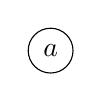
\begin{tikzpicture}
\draw (0,0) node[circle, draw] {$a$} ;
\end{tikzpicture}
\end{center}
and given trees $t_1,t_2$, the tree corresponding to $[t_1,t_2]$ is given by forming a tree with a root and two branches, pasting $t_1$ onto the left branch, and pasting $t_2$ onto the right branch:
\begin{center}
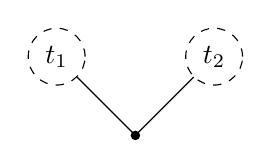
\begin{tikzpicture}
\draw (-1,1) node[circle, dashed, draw](t1) {$t_1$} ;
\draw (1,1) node[circle, dashed, draw](t2) {$t_2$} ;
  \draw[fill=black] (0,0) circle[radius=1.5pt] coordinate(root) ;
\draw (t1) -- (root) -- (t2) ;
\end{tikzpicture}
\end{center}

By \Cref{thmUniquenessOfInductivelyDefinedSets}, there is a unique bijection $A \to T$ that is compatible with the constructors in each set. For example, the element $[[[a_1,a_2],a_3],[a_4,a_5]] \in A$ corresponds with the following tree:
\begin{center}
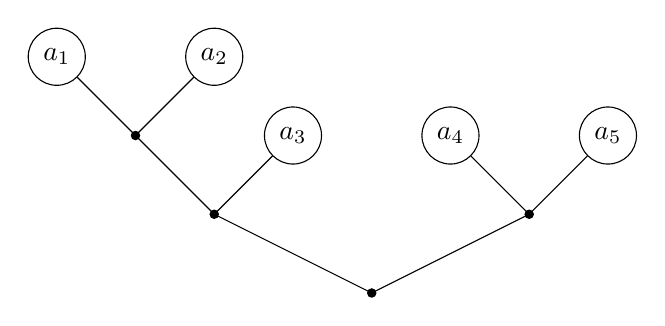
\begin{tikzpicture}
\draw[fill=black] (0,0) circle[radius=1.5pt] coordinate(root) ;
  \draw[fill=black] (-2,1) circle[radius=1.5pt] coordinate(rabc) ;
    \draw[fill=black] (-3,2) circle[radius=1.5pt] coordinate(rab) ;
      \draw (-4,3) node[circle, draw](a) {$a_1$} ;
      \draw (-2,3) node[circle, draw](b) {$a_2$} ;
    \draw (-1,2) node[circle, draw](c) {$a_3$} ;
  \draw[fill=black] (2,1) circle[radius=1.5pt] coordinate(rde) ;
    \draw (1,2) node[circle, draw](d) {$a_4$} ;
    \draw (3,2) node[circle, draw](e) {$a_5$} ;
\draw (root) -- (rabc) -- (rab) -- (a) ;
                    \draw (rab) -- (b) ;
          \draw (rabc) -- (c) ;
\draw (root) -- (rde) -- (d) ;
          \draw (rde) -- (e) ;
\end{tikzpicture}
\end{center}
\end{example}

\subsection*{\optmark{Quotient-inductive sets}}

Some sets appear to be inductively defined, in the sense that its elements can be constructed from some basic elements by applying some constructors, except there may be more than one way of expressing each of its elements as a constructor applied to some elements of the set.

For example, consider the set $\mathbb{Z}$ of integers. Every integer $n$ can be obtained from $0$ by either adding $1$ or subtracting $1$ some number of times. Thus we'd like to say that $\mathbb{Z}$ is inductively defined by the rules
\[ (~ \mid 0) \quad s = (x \mid x+1) \quad p = (x \mid x-1) \]
Here $s$ stands for `successor' and $p$ stands for `predecessor'. However, strictly 	speaking, $\mathbb{Z}$ is not inductively defined by these rules; for example
\[ 2 = 1 + 1 = f_s(1) \quad \text{and} \quad 2 = 3 - 1 = f_p(3) \]
and so $2$ does not have a \textit{unique} expression as a constructor applied to an integer.

In fact, the inductively defined set $A$ generated by the three rules above consists of all strings of the form
\[ 0 \pm 1 \pm 1 \pm \cdots \pm 1 \]
with each $\pm$ sign being either $+$ or $-$. We recover the corresponding integer by evaluating the string; this evaluation function defines a \textit{surjection} $q : A \to \mathbb{Z}$; for example
\[ q(0+1+1) = 2 \quad \text{and} \quad q(0+1+1+1-1+1-1-1+1) = 2 \]
As made precise in \Cref{thmEquivalenceRelationsSurjections}, the fact that there is a surjection $A \to \mathbb{Z}$ means that we can think of $\mathbb{Z}$ as being a quotient of $A$ by a suitable equivalence relation.

To see what this equivalence relation is, note that $(n+1)-1 = n$ and $(n-1)+1=n$ for all $n \in \mathbb{Z}$. Thus in a string $0 \pm 1 \pm \cdots \pm 1$, we can add or remove instances of `$+1-1$' or `$-1+1$' in the string as we please, and we will obtain the same integer. So define an equivalence relation $\sim$ on $A$ by letting $a \sim b$ if and only if the string $b$ can be obtained from $a$ by adding or removing `$+1-1$' or `$-1+1$' some number of times; for example
\[ 0+1+1 \quad \sim \quad 0+1-1+1+1 \quad \sim \quad 0+1+1+1-1+1-1-1+1 \]
Then $\sim$ is an equivalence relation on $A$, and the evaluation function $q : A \to \mathbb{Z}$ descends to a bijection $\bar q : A/{\sim} \to \mathbb{Z}$.

We will call sets obtained in this way \textit{quotient-inductive sets}.

\begin{definition}
\label{defFunctionRespectsRule}
Let $A$ be an inductively defined set and let $\sigma$ be a rule. A function $h : A \to X$ with domain $A$ \textbf{respects} $\sigma$ if, for all $\mathbf{a},\mathbf{b} \in A^{\mathrm{ar}(\sigma)}$, we have
\[ [\forall i \in [\mathrm{ar}(\sigma)],~ h(a_i) = h(b_i)] \quad \Rightarrow \quad h(f_{\sigma}(\mathbf{a})) = h(f_{\sigma}(\mathbf{b})) \]
\end{definition}

\todo{Example, exercise}

\begin{definition}
\label{defQuotientInductiveSet}
\index{set!quotient-inductive}
\index{quotient!quotient-inductive set}
\index{inductively defined set!quotient-inductive}
A \textbf{quotient-inductive set} is a set $Q$ equipped with a surjection $q : A \to Q$ for some inductively defined set $A$, such that $q$ respects all of the rules of $A$.

The function $q$ is called the \textbf{quotient map}; the \textbf{basic elements}, \textbf{constructors} and \textbf{rules} of $Q$ are the images under $q$ of those of $A$.
\end{definition}

We will abuse notation slightly in the following way. Given a rule $\sigma$ and $\mathbf{u} \in Q^{\mathrm{ar}(\sigma)}$, we will write $f_{\sigma}(\mathbf{u})$ instead of $q(f_{\sigma}(\mathbf{a}))$, where $\mathbf{a} \in A^{\mathrm{ar}(\sigma)}$ is such that $q(a_i) = u_i$ for each $i \in [\mathrm{ar}(\sigma)]$. Note that this is well-defined: the elements $a_i$ for $i \in [\mathrm{ar}(\sigma)]$ exist since $q$ is surjective, and the value of $q(f_{\sigma}(\mathbf{a}))$ is independent on the choices of $a_i$ picked since $q$ respects the rules of $A$.

\begin{example}
As we discussed, the rules $(~ \mid 0)$, $s = (x \mid x+1)$ and $p = (x \mid x-1)$ give rise to an inductively defined set $A$ whose elements are strings of the form $0 \pm 1 \pm 1 \pm \cdots \pm 1$, with each `$\pm$' sign replaced with either $+$ or $-$.

The function $q : A \to \mathbb{Z}$ given by evaluating the string is evidently a surjection: indeed, given $n \in \mathbb{Z}$, if $n \ge 0$ then $n = q(0+\underbrace{1+\cdots+1}_{\text{$n$ `$1$'s}})$, and if $n < 0$ then $n = q(0-\underbrace{1-\cdots-1}_{\text{$|n|$ `$1$'s}})$.

Thus $\mathbb{Z}$ is a quotient-inductive set, with basic element $0$ and constructors `$+1$' and `$-1$'.
\end{example}

\begin{exercise}
Prove that the set $\mathbb{Z}^+$ of all positive integers is a quotient-inductive set given by the rules $(~ \mid 1)$ and $(x \mid x \cdot p)$ for each positive prime $p \in \mathbb{Z}$. Describe the corresponding inductively defined set $A$ and the quotient map $q : A \to \mathbb{Z}^+$ explicitly.
\end{exercise}

The reason we generalise the notion of an inductively defined set to that of a quotient-inductive set is that we can generalise the structural induction principle to such sets.

Note, however, that the structural recursion theorem depends in an essential way on the uniqueness of the representation of elements in terms of constructors, so we cannot expect the structural recursion theorem to generalise to quotient-inductive sets.

\begin{theorem}[Structural induction principle for quotient-inductive sets]
\label{thmStructuralInductionForQuotientInductiveSets}
\index{induction!structural (for quotient-inductive sets)}
\index{structural induction!for quotient-inductive sets}
Let $Q$ be a quotient-inductive set and let $p(x)$ be a logical formula with free variable $x \in Q$. If for all rules $\sigma$ and all $\mathbf{x} \in Q^{\mathrm{ar}(\sigma)}$ we have
\[ [\forall i \in [\mathrm{ar}(\sigma)],~ p(x_i)] \Rightarrow p(f_{\sigma}(\mathbf{x})) \]
then $p(x)$ is true for all $x \in Q$.
\end{theorem}

\begin{cproof}
Let $q : A \to Q$ be the quotient map from the inductively defined set $A$, and let $\overline{p}(x)$ be the logical formula with free variable $x \in A$ defined by letting $\overline{p}(x)$ mean $p(q(x))$.

Since $q$ is surjective, if $\overline{p}(x)$ is true for all $x \in A$, then $p(x)$ is true for all $x \in Q$. But the assumptions in the statement of the theorem imply that for all rules $\sigma$ we have
\[ \forall \mathbf{x} \in A^{\mathrm{ar}(\sigma)},~ [\forall i \in [\mathrm{ar}(\sigma)],~ \overline{p}(x_i)] \Rightarrow \overline{p}(f_{\sigma}(\mathbf{x}) \]
and so $\overline{p}(x)$ is true for all $x \in A$ by (the usual version of) structural induction on $A$.
\end{cproof}

\index{induction!structural|)}
